\section{Uppgift 3}\label{sec:uppg03}

\subsection{Instruktioner}
\begin{verbatim}
3. Skriv en klass Cirkel som representerar en cirkel. I klassen ska följande
   två instansvariabler ingå:

   radie (int), färg (String)

   I parentes står lämplig datatyp.

   I klassen ska finnas en metod för var och en av följande operationer:

   - ändra färgen på cirkeln
   - returnera cirkelns färg
   - ändra cirkelns radie
   - returnera cirkelns radie
   - beräkna och returnera cirkelns omkrets
   - beräkna och returnera cirkelns area


   När man ska initiera ett cirkel-objekt ska man kunna välja på följande två
   alternativ:

   - välja *både* färg och radie på cirkeln
   - välja endast radien på cirkeln, men cirkelns färg blir alltid gul

   Detta betyder att du behöver två stycken konstruktorer (som överlagrar
   varandra) i din klass.

   Slutligen skriv ett testprogram som testar så att klassens metoder fungerar
   som de ska.  Skapa åtminstone två stycken cirkel-objekt, som använder sig av
   olika konstruktorer. Alla decimaltals-utskrifter på skärmen ska avrundas
   till *en* decimal.

   Tips: För att vid utskrift avrunda ett decimaltal använd klassen
   DecimalFormat, finns exempel i boken hur du använder denna. Den ligger i
   paketet java.text, du måste alltså importera denna klass i ditt testprogram.
\end{verbatim}


\subsection{Källkod}
\javacode{src/Lab3Uppg03/Lab3Uppg03.java}
\caption{Lab3Uppg03.java}
\label{src:uppg03}

\javacode{src/Lab3Uppg03/Cirkel.java}
\caption{Cirkel.java}
\label{src:cirkel}


\subsection{Skärmdump}
\begin{figure}[htbp]
    \centering
        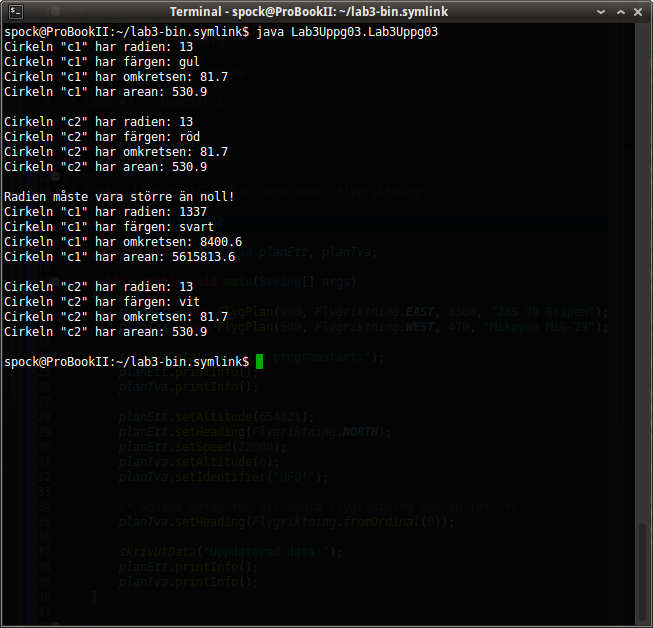
\includegraphics[width=\linewidth]{img/03.png}
    \caption{Körning av koden till Uppgift~\ref{sec:uppg03}}
    \label{fig:uppg03-screenshot}
\end{figure}

